\documentclass[]{article}
\usepackage[utf8]{inputenc}
\usepackage{graphicx} % the demo option is just for the example
\usepackage{amssymb}
\usepackage{titling}
\usepackage[section]{placeins}
\usepackage{listings}


\newcommand{\subtitle}[1]{%
	\posttitle{%
		\par\end{center}
	\begin{center}\large#1\end{center}
	\vskip0.5em}%
}
\pretitle{%
	\begin{center}
		\LARGE
		
\includegraphics[width=10cm]{feup.png}\\[\bigskipamount]
		\vspace{50px}
	}
\posttitle{\end{center}}

% Title Page
\title{A hands-on approach on botnets for a learning proposal\\}
\subtitle{
	Computer Systems Security (EIC0072)
}
\author{Eduardo José Valadar Martins (ei11104@fe.up.pt)\\
	João Pedro Matos Teixeira Dias (ei11137@fe.up.pt)\\
	José Pedro Vieira de Carvalho Pinto (ei12164@fe.up.pt)\\
	João Carlos Teixeira de Sá (ei11142@fe.up.pt)\\\\Group 6 - Theme 12\\
}

\begin{document}
\maketitle
\thispagestyle{empty}
\newpage

\tableofcontents
\newpage
\section{Introduction}

A botnet is, by definition, the name given to any collection of compromised hosts (PCs) controlled by an attacker remotely. Botnets generally are created by a specific attacker or small group of attackers using one piece of malware to infect a large number of machines. The individual machines that are part of the botnet are, generally, called \textit{bots}, \textit{nodes} or \textit{zombies}. There are botnets of various sizes (there is no minimum number of infected machines to the group be called a botnet), and they can vary from small ones with hundreds or low thousands of infected machines and larger ones with millions of compromised hosts \cite{website:botnet-def}.

There are specific cases where bots perform beneficial and even vital activities \cite{website:botnet-useful}, for example, the use of web crawlers by search engines to index web-pages can be considered as a type of bot, also, the participants of SETI@home initiative (Search for Extraterrestrial Intelligence), are, voluntary, part of a large botnet used to analyze radio telescope data in order to track evidence of intelligent extraterrestrial life \cite{website:setihome}.

Attackers usually install bots by exploiting vulnerabilities in software or by using social engineering tactics to trick users into installing malware. Users are often unaware that their computers are being used for malicious purposes \cite{website:botnet-useful}.

Botnets can be used for various activities but the most traditional and common use is for DDoS (Distributed Denial of Service) attacks. These attacks rely on the computing power and bandwidth of hundreds or thousands of PCs to send huge amounts of traffic at a specific Web site in an effort to knock the site offline. Other uses for botnets are, for example, spamming, sniffing traffic, keylogging and even manipulating online polls and games \cite{article:honeypot-tracking}. 

As of today, we think that it's essential that there is a simple way to learn about botnets, what they are, how they work and what we can do about it. For that we built a two modules project. The first one consists of a \textit{wiki} with information regarding botnets, its anatomy, architecture and impact on the technological world. The second part is a more technical one, consisting on a laboratory with a simple and open-source botnet kit with a set of built-in functionalities for anyone who is interested and want to setup a laboratory at home and play with it, finding out how can it be changed and adapted for almost anything.

\section{Research and background}

\subsection{Botnet anatomy}

The term botnet is widely used when several IRC bots have been linked and may possibly set channel modes on other bots and users while keeping IRC channels free from unwanted users. This is where the term is originally from, since the first illegal botnets were similar to legal botnets.

Botnets sometimes compromise computers whose security defenses have been breached and control conceded to a third party. Each such compromised device, known as a “bot”, is created when a computer is penetrated by software from a malware (malicious software) distribution. However, it could also be someone (or a spider) that hacks into a computer. The controller of a botnet is able to direct the activities of these compromised computers through communication channels formed by standards-based network protocols such as IRC or Hypertext Transfer Protocol (HTTP) \cite{article:sans}.

After successful exploitation, a bot uses Trivial File Transfer Protocol (TFTP), File Transfer Protocol (FTP), HyperText Transfer Protocol (HTTP), or CSend (an IRC extension to send files to other users, comparable to DCC) to transfer itself to the compromised host. The binary is started, and tries to connect to the hard-coded master IRC server. Often a dynamic DNS name is provided rather than a hard coded IP address, so the bot can be easily relocated. Some bots even remove themselves if the given master server is localhost or in a private subnet, since this indicates an unusual situations. 

Once an attacker is in control of the bots, they can do whatever they want with the bots: Searching for sensitive information on all compromised machines and DCC-sending these files to another machine, DDoS-ing individuals or organizations, or enabling a keylogger and looking for PayPal or eBay account information. These are just a few possible commands, other options have been presented in the previous section. The IRC server that is used to connect all bots is in most cases a compromised box. This is probably because an attacker would not receive operator-rights on a normal chat network and thus has to set-up their own IRC server which offers more flexibility.

\subsubsection{Organization}

A botnet’s originator (known as a “bot herder” or “bot master”) can control the group remotely, usually through IRC, and often for criminal purposes. Though rare, more experienced botnet operators program command protocols from scratch. These protocols include a server program, a client program for operation, and the program that embeds the client on the victim’s machine. This server is known as the command-and-control (C\&C) server. The bots communicate over a network, using a unique encryption scheme for stealth and protection against detection or intrusion into the botnet.

A bot typically runs hidden and uses a covert channel to communicate with its C\&C server. Generally, the perpetrator has compromised multiple systems using various tools (exploits, buffer overflows, as well as others; see also RPC). Newer bots can automatically scan their environment and propagate themselves using vulnerabilities and weak passwords. Generally, the more vulnerabilities a bot can scan and propagate through, the more valuable it becomes to a botnet controller community. The process of stealing computing resources as a result of a system being joined to a “botnet” is sometimes referred to as “scrumping.”

A few important aspects about to note how botnets have countered measures against them are:

\begin{itemize}
	\item Botnet servers are typically redundant, linked for greater redundancy so as to reduce the threat of a takedown. Actual botnet communities usually consist of one or several controllers that rarely have highly developed command hierarchies; they rely on individual peer-to-peer relationships\cite{article:botcomun}.

	\item Botnet architecture evolved over time, and not all botnets exhibit the same topology for command and control. Advanced topology is more resilient to shutdown, enumeration or discovery. However, some topologies limit the marketability of the botnet to third parties \cite{article:hackbot}. Typical botnet topologies are star, multi-server, hierarchical and random.

	\item Some botnets are scaling back in size to minimize detection. As of 2006, the average size of a network was estimated at 20,000 computers \cite{website:bottrojan}.


\end{itemize}
\subsubsection{Types of botnets}

\begin{itemize}
	\item \textbf{Agobot (parent of Phatbot/Forbot/XtremBot)}

This is probably the best known bot. There are more than 500 known different versions of Agobot and this number is increasing. The bot itself is written in C++ with cross-platform capabilities and the source code is put under the GPL. The latest available versions of Agobot are written in tidy C++ and show a really high abstract design. The bot is structured in a very modular way, and it is very easy to add commands or scanners for other vulnerabilities. Agobot uses libpcap (a packet sniffing library) and Perl Compatible Regular Expressions (PCRE) to sniff and sort traffic. Agobot can use NTFS Alternate Data Stream (ADS) and offers Rootkit capabilities like file and process hiding to hide its own presence on a compromised host. Furthermore, reverse engineering this malware is harder since it includes functions to detect debuggers (e.g. SoftICE and OllyDbg) and virtual machines (e.g. VMWare and Virtual PC). In addition, Agobot is the only bot that utilized a control protocol other than IRC. Furthermore, the Linux version is able to detect the Linux distribution used on the compromised host and sets up a correct init script \cite{article:honeypot-tracking}.

\item \textbf{SDBot (parent of RBot/UrBot/UrXBot/etc.)}

This family of malware is at the moment the most active one. SDBot is written in very poor C and also published under the GPL. It is the father of RBot, RxBot, UrBot, UrXBot, JrBot,.. and probably many more. The source code of this bot is not very well designed or written. Nevertheless, attackers like it, and it is very often used in the wild. It offers similar features to Agobot, although the command set is not as large, nor the implementation as sophisticated \cite{article:honeypot-tracking}.

\item\textbf{ mIRC-based Bots - GT-Bots}

We subsume all mIRC-based bots as GT-bots, since there are so many different versions of them that it is hard to get an overview of all forks. mIRC itself is a popular IRC client for Windows. GT is an abbreviation for Global Threat and this is the common name used for all mIRC-scripted bots. These bots launch an instance of the mIRC chat-client with a set of scripts and other binaries. One binary you will never miss is a HideWindow executable used to make the mIRC instance unseen by the user. The other binaries are mainly Dynamic Link Libraries (DLLs) linked to mIRC that add some new features the mIRC scripts can use. The mIRC-scripts, often having the extension “.mrc”, are used to control the bot. They can access the scanners in the DLLs and take care of further spreading. GT-Bots spread by exploiting weaknesses on remote computers and uploading themselves to compromised hosts \cite{article:honeypot-tracking}.

\end{itemize}

These three last examples of bots are probably the most common ones, in terms of usage and also que more capable ones as for their features and implementation. There are however other types of bots which given their very interesting features are worthy of mentioning in this topic.

\begin{itemize}
\item\textbf{ DSNX Bots}

The Dataspy Network X (DSNX) bot is written in C++ and has a convenient plugin interface. An attacker can easily write scanners and spreaders as plugins and extend the bot’s features. Again, the code is published under the GPL. This bot has one major disadvantage: the default version does not come with any spreaders. But plugins are available to overcome this gap. Furthermore, plugins that offer services like DDoS-attacks, portscan-interface or hidden HTTP-server are available \cite{article:honeypot-tracking}.

\item \textbf{Q8 Bots}

Q8bot is a very small bot, consisting of only 926 lines of C-code. And it has one additional noteworthiness: It’s written for Unix/Linux systems. It implements all common features of a bot: Dynamic updating via HTTP-downloads, various DDoS-attacks (e.g. SYN-flood and UDP-flood), execution of arbitrary commands, and many more. In the version we have captured, spreaders are missing. But presumably versions of this bot exist which also include spreaders \cite{article:honeypot-tracking}.

\item \textbf{kaiten}

This bot lacks a spreader too, and is also written for Unix/Linux systems. The weak user authentication makes it very easy to hijack a botnet running with kaiten. The bot itself consists of just one file. Thus it is very easy to fetch the source code using wget, and compile it on a vulnerable box using a script. Kaiten offers an easy remote shell, so checking for further vulnerabilities to gain privileged access can be done via IRC \cite{article:honeypot-tracking}.

\item \textbf{Perl-based bots}

There are many different version of very simple based on the programming language Perl. These bots are very small and contain in most cases only a few hundred lines of code. They offer only a rudimentary set of commands (most often DDoS-attacks) and are used on Unix-based systems \cite{article:honeypot-tracking}.

\end{itemize}


\subsubsection{Malicious uses of botnets}

A botnet is nothing more than a tool, there are as many different motives for using. The most common uses are criminally motivated or for destructive purposes. The possibilities to use botnets can be categorized as listed below. And since a botnet is nothing more than a tool, there are most likely other potential uses that we have not listed.


\begin{itemize}
	
\item{ \textbf{Distributed Denial-of-Service Attacks}

Often botnets are used for Distributed Denial-of-Service (DDoS[1]) attacks. A DDoS attack is an attack on a computer system or network that causes a loss of service to users, typically the loss of network connectivity and services by consuming the bandwidth of the victim network or overloading the computational resources of the victim system. In addition, the resources on the path are exhausted if the DDoS-attack causes many packets per second (pps). Most commonly implemented and also very often used are TCP SYN and UDP flood attacks \cite{website:ddos}.

Note that DDoS attacks are not limited to web servers, virtually any service available on the Internet can be the target of such an attack. Higher-level protocols can be used to increase the load even more effectively by using very specific attacks, such as running exhausting search queries on bulletin boards or recursive HTTP-floods on the victim’s website. Recursive HTTP-flood means that the bots start from a given HTTP link and then follows all links on the provided website in a recursive way. This is also called spidering \cite{website:ddos}.
}
\item \textbf{Spamming}

Some bots offer the possibility to open a SOCKS v4/v5 proxy - a generic proxy protocol for TCP/IP-based networking applications (RFC 1928[2]) - on a compromised machine. After having enabled the SOCKS proxy, this machine can then be used for nefarious tasks such as spamming. With the help of a botnet and thousands of bots, an attacker is able to send massive amounts of bulk email (spam). Some bots also implement a special function to harvest email-addresses. Often that spam you are receiving was sent from, or proxied through, old Windows computers sitting at home. In addition, this can, of course, also be used to send phishing-mails since phishing is a special case of spam \cite{website:spam} \cite{article:honeypot-tracking}.

\item \textbf{Sniffing Traffic}

Bots can also use a packet sniffer to watch for interesting clear-text data passing by a compromised machine. The sniffers are mostly used to retrieve sensitive information like usernames and passwords. But the sniffed data can also contain other interesting information. If a machine is compromised more than once and also a member of more than one botnet, the packet sniffing allows to gather the key information of the other botnet. Thus it is possible to “steal” another botnet \cite{article:honeypot-tracking}.

\item \textbf{Keylogging}

If the compromised machine uses encrypted communication channels (e.g. HTTPS or POP3S), then just sniffing the network packets on the victim’s computer is useless since the appropriate key to decrypt the packets is missing. But most bots also offer features to help in this situation. With the help of a keylogger it is very easy for an attacker to retrieve sensitive information. An implemented filtering mechanism (e.g. “I am only interested in key sequences near the keyword ‘paypal.com’”) further helps in stealing secret data. And if you imagine that this keylogger runs on thousands of compromised machines in parallel you can imagine how quickly PayPal accounts are harvested \cite{article:honeypot-tracking}.

\item \textbf{Spreading new malware}

In most cases, botnets are used to spread new bots. This is very easy since all bots implement mechanisms to download and execute a file via HTTP or FTP. But spreading an email virus using a botnet is a very nice idea too. A botnet with 10.000 hosts which acts as the start base for the mail virus allows very fast spreading and thus causes more harm. The Witty worm, which attacked the ICQ protocol parsing implementation in Internet Security Systems (ISS) products is suspected to have been initially launched by a botnet due to the fact that the attacking hosts were not running any ISS services \cite{article:honeypot-tracking}.

\item \textbf{Installing Advertisement Addons and Browser Helper Objects (BHOs \cite{website:bho})}

Botnets can also be used to gain financial advantages. This works by setting up a fake website with some advertisements: The operator of this website negotiates a deal with some hosting companies that pay for clicks on ads. With the help of a botnet, these clicks can be “automated” so that instantly a few thousand bots click on the pop-ups. This process can be further enhanced if the bot hijacks the start-page of a compromised machine so that the “clicks” are executed each time the victim uses the browser \cite{article:honeypot-tracking} \cite{website:bho}.

\item \textbf{Google AdSense abuse}

A similar abuse is also possible with Google’s AdSense \cite{website:adsense} program: AdSense offers companies the possibility to display Google advertisements on their own website and earn money this way. The company earns money due to clicks on these ads, for example per 10.000 clicks in one month. An attacker can abuse this program by leveraging his botnet to click on these advertisements in an automated fashion and thus artificially increments the click counter. This kind of usage for botnets is relatively uncommon, but not a bad idea from an attacker’s perspective \cite{article:honeypot-tracking} .


\item \textbf{Attacking IRC Chat Networks}

Botnets are also used for attacks against Internet Relay Chat (IRC) networks. Popular among attackers is especially the so called “clone attack”: In this kind of attack, the controller orders each bot to connect a large number of clones to the victim IRC network. The victim is flooded by service request from thousands of bots or thousands of channel-joins by these cloned bots. In this way, the victim IRC network is brought down - similar to a DDoS attack \cite{article:honeypot-tracking}.

\item \textbf{Manipulating online polls/games}

Online polls/games are getting more and more attention and it is rather easy to manipulate them with botnets. Since every bot has a distinct IP address, every vote will have the same credibility as a vote cast by a real person. Online games can be manipulated in a similar way \cite{article:honeypot-tracking}.

\item \textbf{Mass identity theft}

Often the combination of different functionality described above can be used for large scale identity theft, one of the fastest growing crimes on the Internet. Bogus emails (“phishing mails”) that pretend to be legitimate (such as fake PayPal or banking emails) ask their intended victims to go online and submit their private information. These fake emails are generated and sent by bots via their spamming mechanism. These same bots can also host multiple fake websites pretending to be Ebay, PayPal, or a bank, and harvest personal information. Just as quickly as one of these fake sites is shut down, another one can pop up. In addition, keylogging and sniffing of traffic can also be used for identity theft \cite{article:honeypot-tracking}.


\end{itemize}


This list demonstrates that attackers can cause a great deal of harm or criminal activity with the help of botnets. Many of these attacks – especially DDoS attacks - pose severe threats to other systems and are hard to prevent. In addition, we are sure there are many other uses we have not covered in this list.

\subsubsection{Vulnerabilities exploitation}

In computer security, a vulnerability is defined as: a weakness that allows an attacker to reduce a system’s information assurance. Vulnerability is a intersection of three elements: a system susceptibility or flaw, attacker access to the flaw, and attacker capability to exploit the flaw \cite{article:sans}.

Due to their immense size - botnets can consist of several ten thousand compromised machines - botnets pose serious threats. Distributed denial-of-service (DDoS) attacks are one such threat. Even a relatively small botnet with only 1000 bots can cause a great deal of damage. These 1000 bots have a combined bandwidth (1000 home PCs with an average upstream of 128KBit/s can offer more than 100MBit/s) that is probably higher than the Internet connection of most corporate systems. In addition, the IP distribution of the bots makes ingress filter construction, maintenance, and deployment difficult. In addition, incident response is hampered by the large number of separate organizations involved.

Another use for botnets is stealing sensitive information or identity theft: Searching some thousands home PCs for password.txt, or sniffing their traffic, can be effective. The spreading mechanisms used by bots is a leading cause for “background noise” on the Internet, especially on TCP ports 445 and 135. In this context, the term spreading describes the propagation methods used by the bots. These malware scan large network ranges for new vulnerable computers and infect them, thus acting similar to a worm or virus.

\subsection{History}

The “boom” of the internet and the massive increase of the use of the e-mail made the conditions ideal for the appearance of botnets. In fact, as you will see below, most of the botnets detected until today are somehow related to sending enourmous amounts of e-mails, especially spam. Be aware that the estimated number of bots presented below are just that, estimatives, because in some countries it is common that users change their IP address several times a day.

\begin{itemize}
	\item {2004
\begin{itemize}
	\item \textbf{Bagle} \cite{website:bagle}

	\item \textit{Est. no of bots:} 230 000

	\item Bagle (also known as Beagle) is a mass-mailing computer worm affecting all versions of Microsoft Windows. Bagle uses its own SMTP engine to mass-mail itself as an attachment to recipients. It copies itself to the Windows system directory and opens a backdoor.
\end{itemize}
}

	\item {2006

\begin{itemize}
	\item \textbf{Rustock} \cite{website:rustock}

	\item \textit{Est. no of bots:} 150 000

	\item Rustock botnet consisted of computers running Microsoft Windows and was capable of sending up to 25,000 spam messages per hour from an infected PC. To increase the size of the botnet it would use self-propagation by sending malicious e-mails with a trojan which would incorporate the targeted machine into the botnet.
\end{itemize}
}

	\item {2007

\begin{itemize}
	\item \textbf{Akbot} \cite{website:akbot}

\item \textit{Est. no of bots:} 1 300 000

\item Akbot is an IRC controlled backdoor program that allows an outside user to take control of the infected computer. It operates by joining IRC servers and then waiting for further instructions. Once installed, Akbot can be used to gather data, kill processes, or perform DDOS attacks.

\item \textbf{Cutwail} \cite{website:cutwail}

\item \textit{Est. no of bots:} 1 500 000

\item Cutwail botnet is a botnet mostly involved in sending spam e-mails. Typically, it uses a Trojan component called Pushdo to infect a machine. It affects computers running Microsoft Windows.

\item \textbf{Srizbi} \cite{website:srizbi}

\item \textit{Est. no of bots:} 450 000

\item Srizbi botnet is a botnet mainly involved in sending spam e-mails. It infects computers with the Srizbi trojan, which allows to send spam on command.
\end{itemize}
}

	\item {2008
\begin{itemize}
	\item \textbf{Mariposa} \cite{website:mariposa}

\item \textit{Est. no of bots:} 12 000 000

\item The Mariposa botnet is a botnet mainly involved in cyberscamming and denial of service attacks. It is one of the largest known botnets with up to 12 million unique IP addresses.

\item \textbf{Sality} \cite{website:sality}

\item \textit{Est. no of bots:} 1 000 000

\item Sality is a family of malicious software which infects files on Microsoft Windows systems. Machines infected with Sality are able to communicate over a peer-to-peer (P2P) network for the purpose of relaying spam, proxying of communications, exfiltrating sensitive data, compromising web servers and/or coordinating distributed computing tasks for the purpose of processing intensive tasks (e.g. password cracking).

\item \textbf{Conficker} \cite{website:conficker}

\item \textit{Est. no of bots:} 10 500 000+

\item Conficker, also known as Downup, Downadup and Kido, is a computer worm targeting the Microsoft Windows operating system. The botnet uses flaws in Windows OS software and dictionary attacks on administrator passwords to propagate itself.

\item \textbf{Grum} \cite{website:grum}

\item \textit{Est. no of bots:} 560 000

\item The Grum botnet, also known by its alias Tedroo and Reddyb, was a botnet mostly involved in sending pharmaceutical spam e-mails. It relies on two types of control servers for its operation. One type is used to push configuration updates to the infected computers, and the other is used to tell the botnet what spam emails to send.
\end{itemize}
}

	\item{ 2009

\begin{itemize}
	\item \textbf{BredoLab}

	\item \textit{Est. no of bots:} 30 000 000
	
	\item The BredoLab Botnet, also known by its alias Oficla, was a botnet mostly involved in viral e-mail spam.

\end{itemize}
}

	\item{ 2010

\begin{itemize}
	\item \textbf{Kelihos} \cite{website:kelihos}

	\item \textit{Est. no of bots:} 300 000+

	\item The Kelihos botnet, also known as Hlux, is a botnet mainly involved in the theft of bitcoins and spamming.

	\item \textbf{TDL-4} \cite{website:TDL4}

	\item \textit{Est. no of bots:} 4 500 000+

	\item TDL-4 is a botnet and the name of the rootkit that runs the botnet (also known as Alureon). It infects the master boot record of the target machine, making it harder to detect and remove.

\end{itemize}
}
	\item{ 2011

\begin{itemize}
	\item \textbf{Ramnit} \cite{website:ramnit}

	\item \textit{Est. no of bots:} 3 000 000

	\item Ramnit is a computer worm affecting Windows operating system. The Ramnit botnet was dismantled by Europol and Symantec securities in 2015.

	\item \textbf{ZeroAccess} \cite{website:zeroaccess}
	\item \textit{Est. no of bots:} 2 000 000

\item ZeroAccess, also known as Max++ and/or Sirefef, is a botnet mostly involved in bitcoin mining and click fraud. It uses a Trojan horse computer malware that affects Microsoft Windows operating systems and downloads other malware on an infected machine while remaining hidden by using rootkit techniques.
\end{itemize}
}
\item {2012
\begin{itemize}
	\item \textbf{Nitol} \cite{website:nitol}

	\item \textit{Est. no of bots:} unknown

	\item The Nitol botnet is a botnet mostly involved in spreading malware and distributed denial-of-service attacks. The botnet is mostly prevalent in China where an estimate 85\% of the infections are detected. It was found to be present on systems that came brand-new from the factory, indicating the trojan was installed somewhere during the assembly and manufacturing process.
\end{itemize}
}
	\item{ 2014
\begin{itemize}
	\item \textbf{Semalt (aka Soundfrost)} \cite{website:semalt}

	\item \textit{Est. no of bots:} 300 000+

	\item Semalt is a botnet mainly involved mainly involved in sending spam e-mails. It visits random websites to generate referral and spies on users browsing habits.
\end{itemize}

}
\end{itemize}

This list demonstrates that there has been several botnets that were able to reach a big dimension infecting thousands (or even millions) of machines. Most of the botnets presented were spam sending related but it is also noticeable that there has been an evolution and they tend to do more than just that. Also botnets have become more complex making it harder to dismantle them.

\subsection{Countermeasures}

\subsubsection{Botnet Detection}

Botnet detection deals with the identification of bots in the machine or network so that some sort of remedy can be done.

In recent years botnet detection has been a hot topic in the research community due to increase in the malicious activity. According to the majority of the common characteristic of a bot malwareare related to network activities the bots require some sort of interaction with the command and control servers. Some of the common activities one could monitor to detect botnets are:

\begin{itemize}
	\item \textit{opening of specific ports}
	\item \textit{establishing a number of unwanted network connections}
	\item \textit{downloading and executing files and programs}
	\item \textit{creating new processes with well-known names}
	\item \textit{disabling antivirus software}
\end{itemize}

\textbf{Detection techniques}

Intrusion Detection System (IDS) is an approach for botnet detection that can be either a signature or anomaly-based technique \cite{website:ids}.

\begin{itemize}
	\item{\textbf{Signature-Based}: A signature-based Botnet detection technique uses the signatures of current Botnets for its detection. This method has several advantages, such as very low false alarm rate, immediate detection, easier to implement and there is better information about the type of detected attack. Signature based detection method can only able to detect well known botnets.
		
	Thus, unknown Botnets can’t be detected by this method. Anomaly-based detection techniques are introduced to overcome this drawback.
		}
	\item {\textbf{Anomaly-Based}:
		The idea behind anomaly-based detection approach is to perform botnet detection by considering several different network traffic anomalies, including high network latency, high traffic volume, traffic on unusual ports, and unusual system behavior that could indicate the presence of malicious bots in the network.
		
		Anomaly-based detection techniques are further divided into host-based detection and network-based detection.
		
		A host-based technique is a detection strategy which monitors and analyzes the internals of a computer system instead of network traffics on its external interfaces. In this approach the individual machine is monitored to find any suspicious behavior, including its processing overhead, and access to suspicious files. If suspicious activity is detected the Host Intrusion Detection Systems will alert the user or administrator. It takes a snapshot of existing system files and matches it to the previous snapshot. If the critical system files were modified or deleted, an alert is sent to the administrator to investigate.
		}
\end{itemize}

\subsection{Botnet countermeasures}

Defense against botnets is carried out by application of certain strategies. All the Internet users are responsible for defense, starting from home or business computer users, system administrators, developers, up to web administrators and ISPs. The defense must be considered as a permanent and comprehensive process in which all the activities must be proactive. This is the only way to achieve good results and to protect computers, i.e. Web services/applications against the activities with bad intentions.

Countermeasures against \textit{botnet treats} can be broadly classified into two approaches, namely, technical approaches or social and regulatory approaches \cite{article:countermeasures}.

\begin{itemize}
	\item \textbf{Technical Approach}: Most of botnet countermeasures focus on the commandand-control infrastructure of botnets by filtering botnet related traffic, sinkholing domains with the assistance of DNS registrars or obtaining the shutdown of malicious servers in data centers. The technical botnet defense approach includes Blacklisting, Packet Filtering, Reverse Engineering and Port Blocking \cite{article:countermeasures}.
	
	\item{ \textbf{Blacklisting}: A blacklist may provide single IP addresses of malicious hosts or whole subnets showing suspicious activities. A blacklist can be used to block all traffic from included addresses and also to filter websites with suspicious or proven malicious contents \cite{article:countermeasures}.
	
	For example, the Spamhaus Project provides various real-time lists that assist in identifying and blocking attempts by malicious activities. Spamhaus Block List (SBL) and the Domain Block List (DBL) contain a collection of IP addresses and domain names respectively from which incoming e-mail should not be accepted \cite{article:countermeasures}.
}
	\item \textbf{Packet Filtering}: The packet filtering can be applied at a host, network and ISP level. A typical component that performs packet filtering at host level is a desktop firewall. Its purpose is to monitor the network activities of all active processes. As the amount of traffic at host level is usually manageable, deep-packet inspection is applicable. Often, user or administrator interaction is required to allow or deny network access for certain applications, if no suitable rules have been specified for them yet \cite{article:countermeasures}.
	
	\item\textbf{ Reverse Engineering}: Recovering the functionality of a program without the source code is known as reverse engineering. The malware reverse engineering technique helps in extracting the details of the installation and spreading of malware. The process involves static analysis and dynamic analysis. In case of static analysis, the binary is not executed. This phase deals with the reconstruction of certain aspects of the functionality. The dynamic analysis deals with the execution of the sample. The behavior of the malware can be determined by monitoring the host \cite{article:countermeasures}.
	
	\item \textbf{Port Blocking}: Port blocking is a preventive measure that can be applied by ISPs to reducing the amount of spam mails traversing their network. The use of unauthenticated services via port 25, like direct mail exchange or open relay mail servers is almost exclusively for spam distribution purposes. Hence, blocking port 25 at ISP level has been recommended as best practice \cite{article:countermeasures}.
\end{itemize}

\section{Implementation}

\subsection{Botnet Wiki}

In order to build the \textit{botnet wiki}, to reach the largest number of people, we decided to build a web platform, namely a wiki, based on W3C standards - HTML, CSS and Javascript \cite{website:standards}. To facilitate the addition of content and edition, we used an automatic site building tool designated Jekyll \cite{app:jekyll} and its support to markdown \cite{app:markdown}. 

This part was built with the objective of transmitting all the results from the research on the topic "botnets". The content presented in the wiki is divided in:
\begin{itemize}
	\item\textbf{Anatomy of a botnets}: Describing how bots and botnets work, types of bots and attacks and vulnerability exploitation.
	\item \textbf{History of botnets}: A little of botnet history including the largest botnets and the impact on the technological world.
	\item \textbf{Botnet countermeasures}: Detection and defense techniques against botnets.
	\item \textbf{Botnet Lab}: Instruction on how to use and setup the \textit{botnet laboratory}.
\end{itemize}

\subsection{Botnet Laboratory}

With the intuit of having a real hands-on tool for testing and developing proposes we created a botnet lab framework, a botnet kit based on the IRC communication protocol, with built-in functionalities and an easy way of expanding functionalities, in a framework way.

The botnet built using this laboratory match the general architecture for any botnet based on a Command-and-Control (C\&C) architecture. Our actor is the Bot Herder or Bot Master, it operates using the a special IRC client (that is part of this laboratory), connects to a IRC-Server (in this case a IRCD-Hybrid based one) where all the bots are connected.

Whenever the Bot Herder sends a message to the IRC Server it broadcast it to all the connected bots that executes the requested job.

Special cases are the Spam request and the Screenshot/Webcam request. In the first case, the Spam, to avoid the trouble of setting up a SMTP server on all the bots we use the Mandrill API for sending the e-mail. While this can appear strange, because of centralizing all the traffic on one e-mail sender API with low free quotas and with the risk of the account being blocked, we send the API Key in the request sended to bots in a way that if a Key it’s blocked we can simple send a different API Key on the request sended to the bots. Additionally it’s used the PasteBin Service and it’s “anonymous and hidden file” hability for hosting relevant data like the the e-mail sending list, API Key and Message and the Bot Herder just needs to send to the bots the files URL (fig.\ref{fig:spam}).

In the second case, the Screenshot/Webcam, the bots uses the Imgur API for storage the images and just send the URL of that images back to the \textit{Bot Herder} (fig.\ref{fig:webcam}).

Adding to all of this, it is used the freegeoip and Google Static Map API for getting and showing the relative world position of the controlled hosts (fig.\ref{fig:location}).

Also, it’s used RSA encryption \cite{article:rsa} so the Bot Herder it’s the only one capable of decrypt the messages sended by the bots because it’s the Private Key owner. The bots encrypts the messages using the Public Key defined by the Bot Herder.

\subsubsection{Technologies}

For setting up the IRC server we used \textit{IRCd-hybrid} - “\textit{A lightweight, high-performance internet relay chat daemon.}”\cite{app:ircdhybrid}.

In order to build the bots we used Python 2.7 \cite{app:python} with the help of some libraries.

Additionally it were the need of build a \textit{special} IRC client, and we used Python too.

Besides this, we used several external API's, namely:

\begin{itemize}
	\item \textbf{freegeoip}: provides a public HTTP API for software developers to search the geolocation of IP addresses. It uses a database of IP addresses that are associated to cities along with other relevant information like time zone, latitude and longitude \cite{app:freegeoip}.
	\item \textbf{Google Static Map API}: create any map based on URL parameters sent through a standard HTTPS request \cite{app:maps}.
	\item \textbf{Mandrill}: is a reliable, scalable, and secure delivery API for transactional emails from websites and applications \cite{app:mandrill}.
	\item \textbf{Pastebin}: a website where we can store text for a certain period of time \cite{app:pastebin}. 
	\item \textbf{imgur API}: an image storage website \cite{app:imgur}.
\end{itemize}

All the developed objects, namely the client and the bot are cross-platform capable of running on Windows and Linux machines. The exception goes to the IRCd-Hybrid server that needs a Linux machine to work.

\subsubsection{Architecture}

The principal network components that interact with the botnet are listed showed in fig.\ref{fig:network}.

\begin{figure}
	\centering
	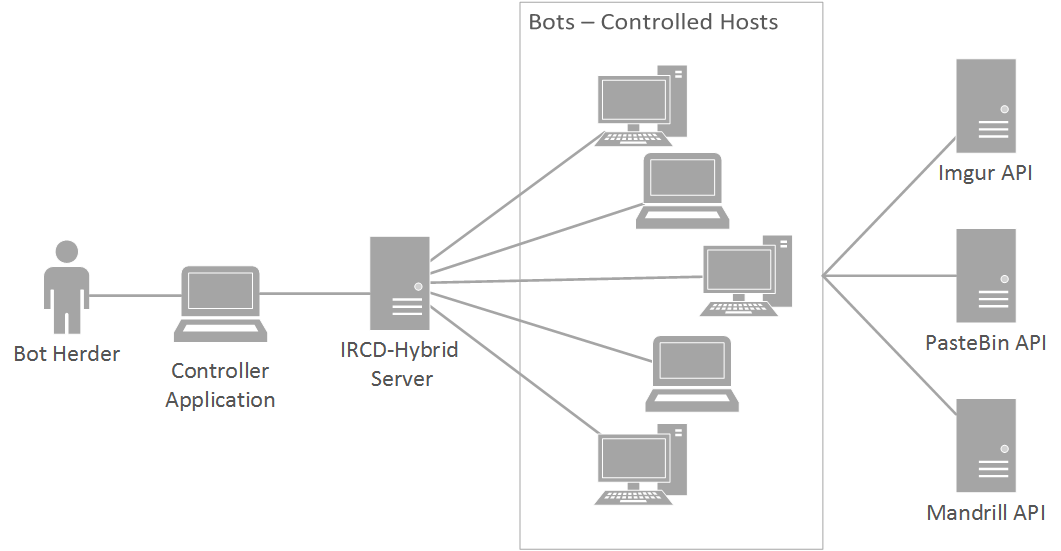
\includegraphics[width=1\textwidth]{network_diagram.png}
	\caption{Network Diagram}
	\label{fig:network}
\end{figure}


A typical communication that can be observed after a successful bot deploy looks like:

\begin{lstlisting}
<- :irc1.XXXXXX.XXX NOTICE AUTH :*** Looking up your hostname
<- :irc1.XXXXXX.XXX NOTICE AUTH :*** Found your hostname
-> PASS secretserverpass
-> NICK [urX]-700159
-> USER mltfvt 0 0 :mltfvt
<- :irc1.XXXXXX.XXX NOTICE [urX]-700159 :*** If you are having 
problems connecting due to ping timeouts, please type /quote 
pong ED322722 or /raw pong ED322722 now.
<- PING :ED322722
-> PONG :ED322722
<- :irc1.XXXXXX.XXX 001 [urX]-700159 :Welcome to the irc1.XXXXXX
 IRC Network
 [urX]-700159!mltfvt@nicetry
<- :irc1.XXXXXX.XXX 002 [urX]-700159 :Your host is irc1.XXXXXX,
 running version IRCd-Hybrid
<- :irc1.XXXXXX.XXX 003 [urX]-700159 :This server was created
 Set  8 18:58:31 2015
<- :irc1.XXXXXX.XXX 004 [urX]-700159 irc1.XXXXXX.XXX IRCd-Hybrid
 iowghraAsORTVSxNCWqBzvdHtGp lvhopsmntikrRcaqOALQbSeKVfMGCuzN
\end{lstlisting}

Afterwards, the server accepts the bot as a client and sends him RPL\_ISUPPORT, RPL\_MOTDSTART, RPL\_MOTD, RPL\_ENDOFMOTD or ERR\_NOMOTD. Replies starting with RPL\_ contain information for the client, for example RPL\_ISUPPORT tells the client which features the server understands and RPL\_MOTD indicates the Message Of The Day (MOTD). In contrast to this, ERR\_NOMOTD is an error message if no MOTD is available.

On RPL\_ENDOFMOTD or ERR\_NOMOTD, the bot will try to join his master’s channel with the provided password:

\begin{lstlisting}
-> JOIN #botnet channelpassword
-> MODE [urX]-700159 +x
\end{lstlisting}

After this the bots keep listening for commands sent by the \textit{Bot Herder}. This communication is showed in fig.\ref{fig:sequential}.


\begin{figure}
	\centering
	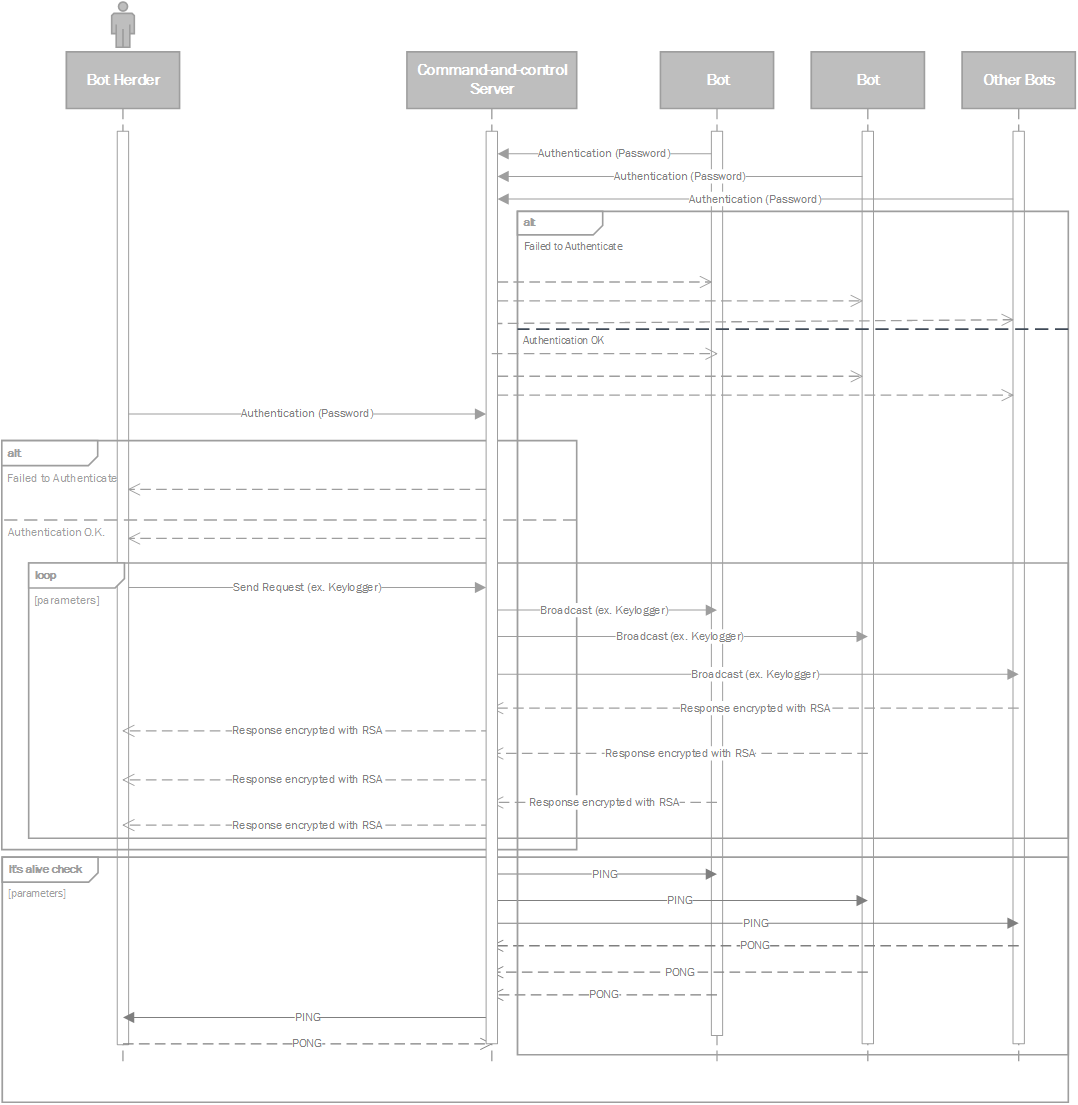
\includegraphics[width=1\textwidth]{sequencial_diagram.png}
	\caption{Basic use sequential diagram.}
	\label{fig:sequential}
\end{figure}


\begin{figure}
	\centering
	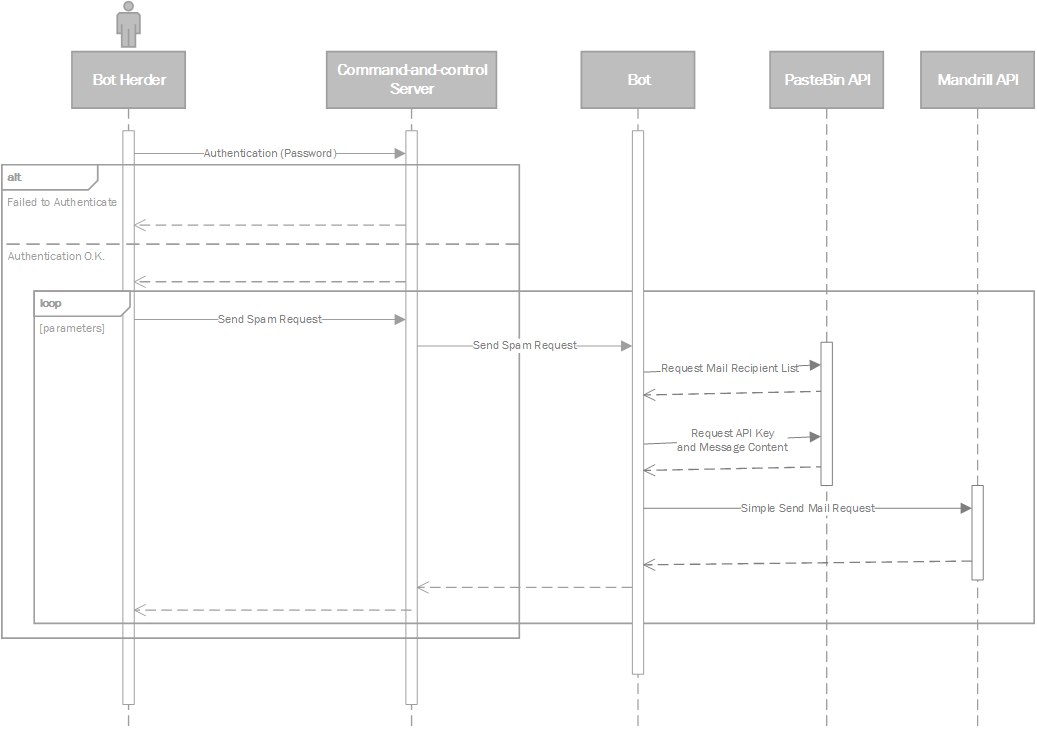
\includegraphics[width=0.85\textwidth]{sequencial_spam_diagram.png}
	\caption{Spam case sequential diagram}
	\label{fig:spam}
\end{figure}


\begin{figure}
	\centering
	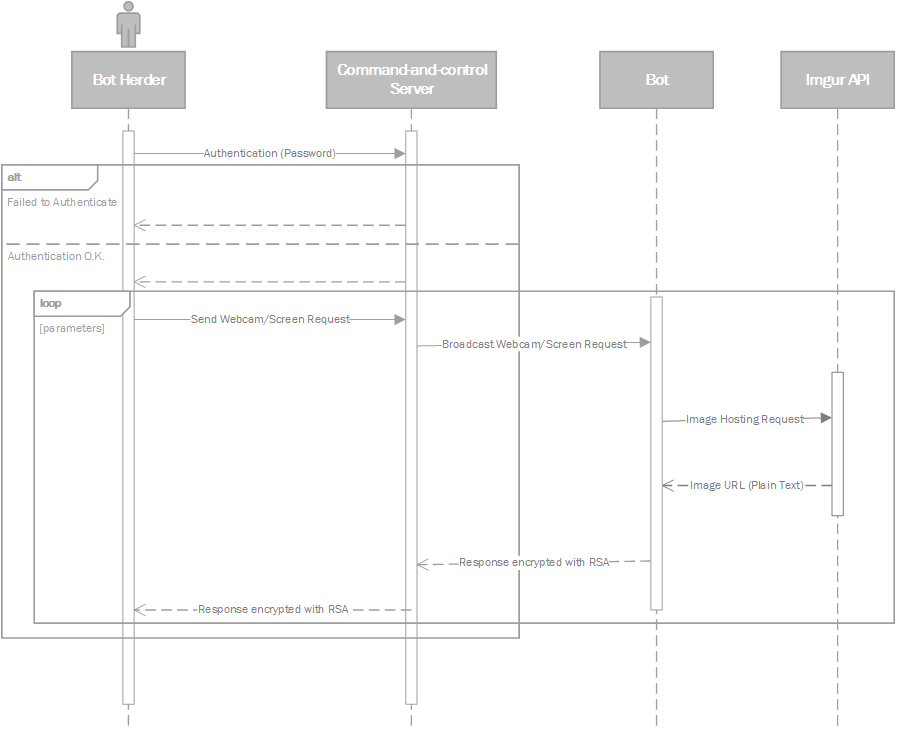
\includegraphics[width=0.85\textwidth]{sequencial_webcam_diagram.png}
	\caption{Webcam/Screenshot case sequential diagram.}
	\label{fig:webcam}
\end{figure}


\begin{figure}
	\centering
	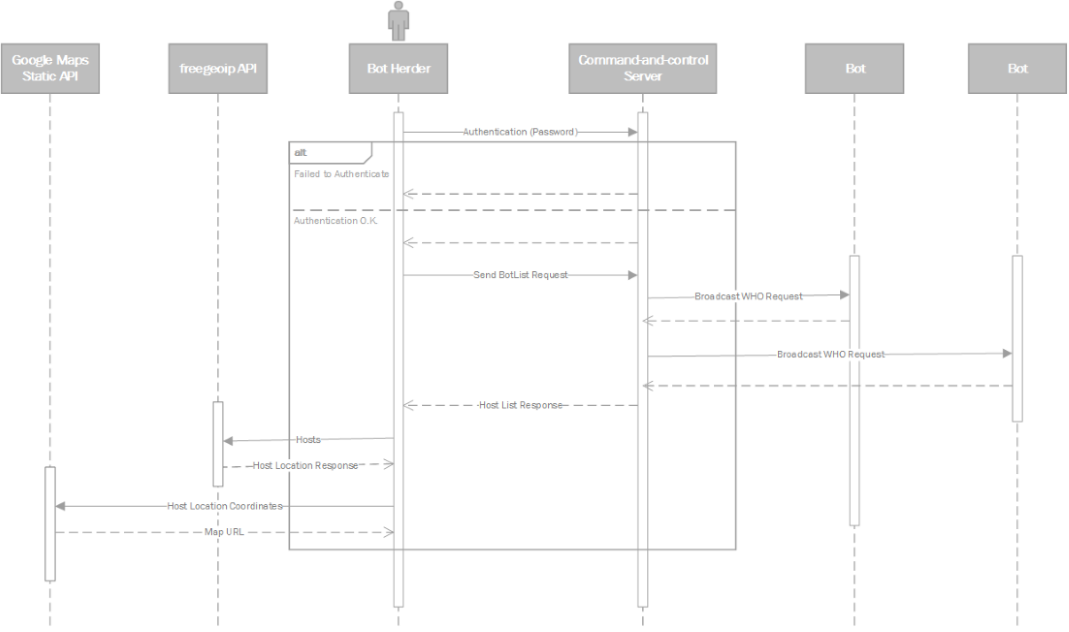
\includegraphics[width=0.85\textwidth]{location_diagram.png}
	\caption{Location request case sequential diagram.}
	\label{fig:location}
\end{figure}


\section{Conclusion and Further Work}

Botnets are a big issue in computer security being responsible for sending huge amounts of spam and being involved in many cybercrimes including DDoS. 

As a result of our research work we present a complete wiki that encompasses the anatomy of a botnet, a list of botnets created along the history and some countermeasures against them making it a useful guide for any person who wants to know more about botnets. As a future work we would like to refer the maintenance of the information presented in it.

We also constructed a very useful tool for anyone who wants to try some features related to botnets. This tool includes all the functionalities that we referred in our initial proposal.

It's also important to refer that all the functionalities, both of wiki and the lab, are working and in the case of the lab there is even support for different operating systems (Linux and Windows).

Also, an important note, all the project and its development was and will be in the future completely open-source, hosted on GitHub, because it represents the idea behind our initial proposal for a learning tool for everyone. The wiki will also be openly available for viewing proposes as well as to ease addition of contributions and improve maintenance.

So, in conclusion, we present a complete work that allies the theory and the practice where the wiki complements the lab work.


\subsubsection{Further Work}

There is, however, some future work that can be done and was not possible due to time limitations.

First off, the wiki could of course be further developed in terms of design quality and content quantity. Also maintaining the information present would also enhance the wiki itself given that botnet’s information changes at a relative great speed.
Next, and most obvious, for the lab, the addition of some out-of-the-box functionalities beside the existing ones. Following that, we had the intention of exploiting any given vulnerability but since that was not covered it would be a good opportunity for future work to do so.
Security of the system, besides using the RSA encryption for communication, is still a priority, so later on, enhancement of the communication channel as well as every other aspect that protects the module against external entities is something to certainly work on.

Given the nature of this tool we’ve developed, it is only appropriate that we improve the whole setup of the environment to easy the experience. In addition, facilitate the addition of new functionalities and the personalization of every possible setting. And final but also important, removing deprecated dependencies and upgrading the whole system from Python 2.7 to 3, which is crucial to a healthy and maintainable piece of software.

\newpage
\bibliographystyle{ieeetrans}
\bibliographystyle{unsrt}
\bibliography{resources} 
 

\end{document}